\documentclass[12pt]{article}
\usepackage[a4paper, left=3.17cm, right=3.17cm, top=2.54cm, bottom=2.54cm]{geometry}
\usepackage[fontset=mac]{ctex}
\usepackage[T1]{fontenc}
\usepackage{mathptmx}
\usepackage{amsfonts}
\usepackage{amsmath,amssymb,amsthm}
\usepackage{enumerate}
\usepackage{graphics}
\usepackage{chemformula}
\usepackage{cite}
\usepackage[colorlinks, linkcolor=black, anchorcolor=black, citecolor=black]{hyperref}
\usepackage{indentfirst}

\usepackage{graphicx}
\setlength{\parskip}{0.5em}
\title{《高性能计算引论》第二次作业}
\author{\textup{罗文水}}
\begin{document}
	
	\begin{titlepage}
		\newcommand{\HRule}{\rule{\linewidth}{0.5mm}}
		\begin{center}
			
\includegraphics[width=8cm]{../HPC_P1/title}			
		\end{center}
		
		\center 
		\quad\\[1.5cm]
		\textsl{\Large \textbf{Nanjing University of Science and Technology} }\\[0.5cm] 
		\textsl{\large School of Computer Science and Engineering}\\[0.5cm] 
		\makeatletter
		\HRule \\[0.4cm]
		{ \huge \bfseries \@title}\\[0.25cm] 
		\HRule \\[1.5cm]
	\begin{minipage}{0.42\textwidth}
		\begin{flushleft}
			
			\Large{\emph{姓名:罗文水}}
			\\
			\Large{\emph{学号:918106840738}}
			\\
			\Large{\emph{班级:计科一班}}
			\\
			\Large{\emph{课程:高性能计算引论}}
			\\
			\Large{\emph{授课教师:李翔宇}}
			\\
		\end{flushleft}
	\end{minipage}
		\vspace{7em} 
		
		{\large \today}\\[2cm] 
		\vfill 
	\end{titlepage}
	
	\newpage
\section{问题一}
	该网络的各项参数如下所示:
	\begin{enumerate}
		\item \textbf{网络直径}
		\item \textbf{等分宽度}
		\item \textbf{边连通度}
	\end{enumerate}
\newpage
\section{问题二}
		(1)运行Hello World程序三次得到的结果分别如下所示。
		\begin{figure}[htbp]
			\centering
			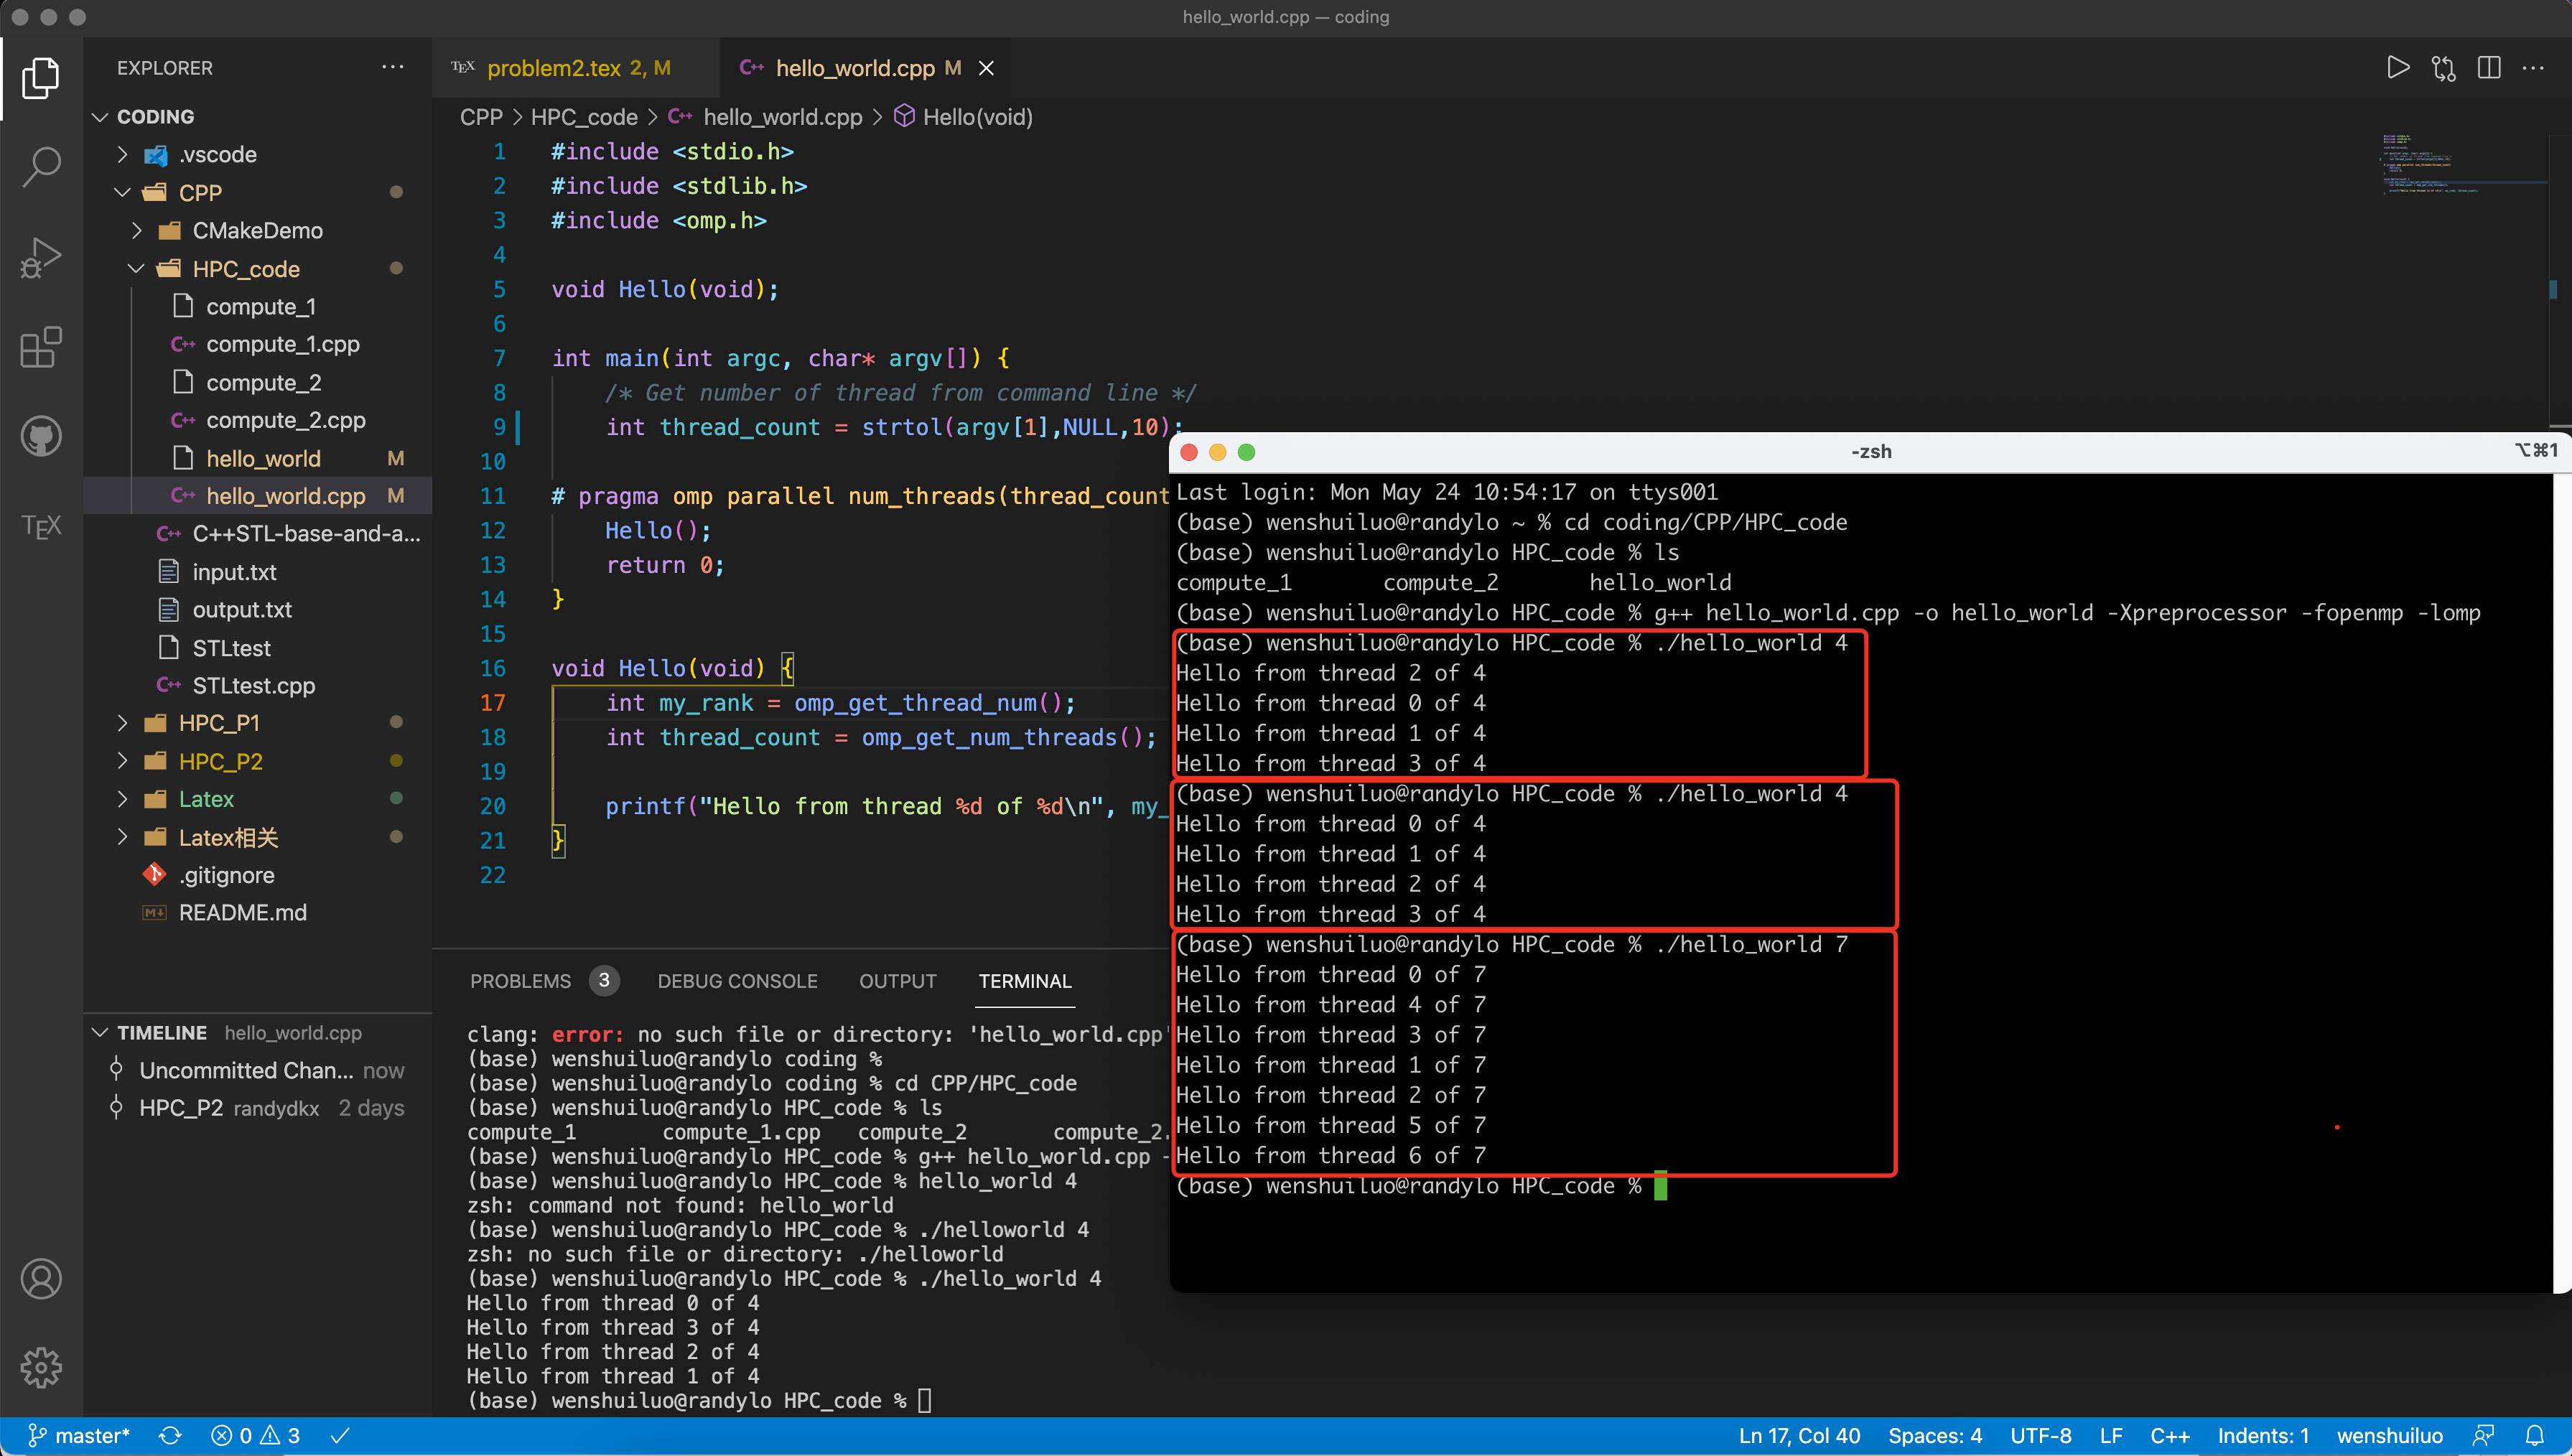
\includegraphics[width=0.9\textwidth]{hello_world三次运行.png}
			\caption{问题一三次运行截图1}
			\label{fig:pro2_1_1}
		\end{figure}
		\begin{figure}[htbp]
			\centering
			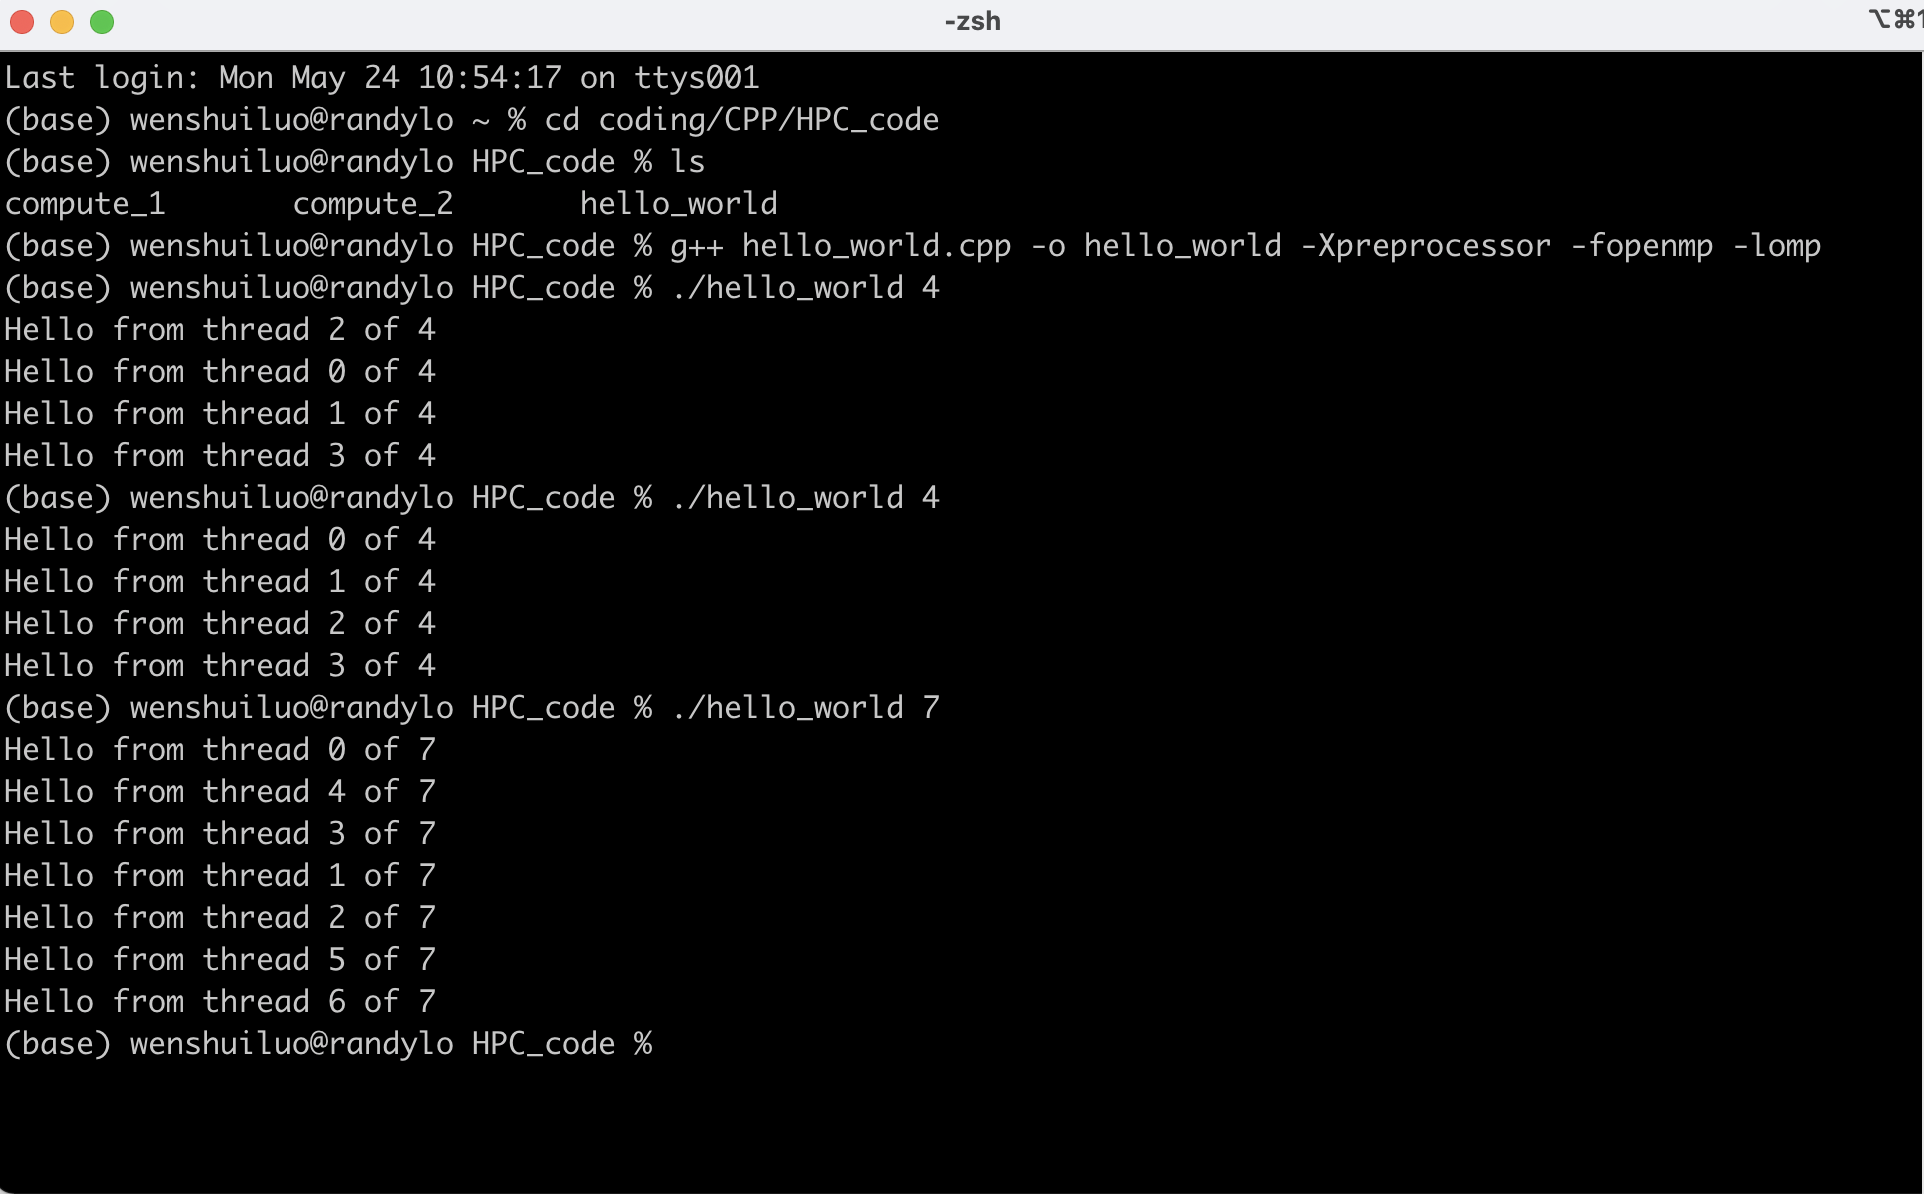
\includegraphics[width=0.9\textwidth]{pro1.png}
			\caption{问题一三次运行截图2}
			\label{fig:pro2_1_2}
		\end{figure}

		从图1和图2中可知三次运行hello world程序分别启动了4、4、7个线程,对于每次执行,每个线程都执行打印hello\_world程序。		

		(2) 两段程序的执行结果分别如下图所示
		\begin{figure}[htbp]
			\centering
			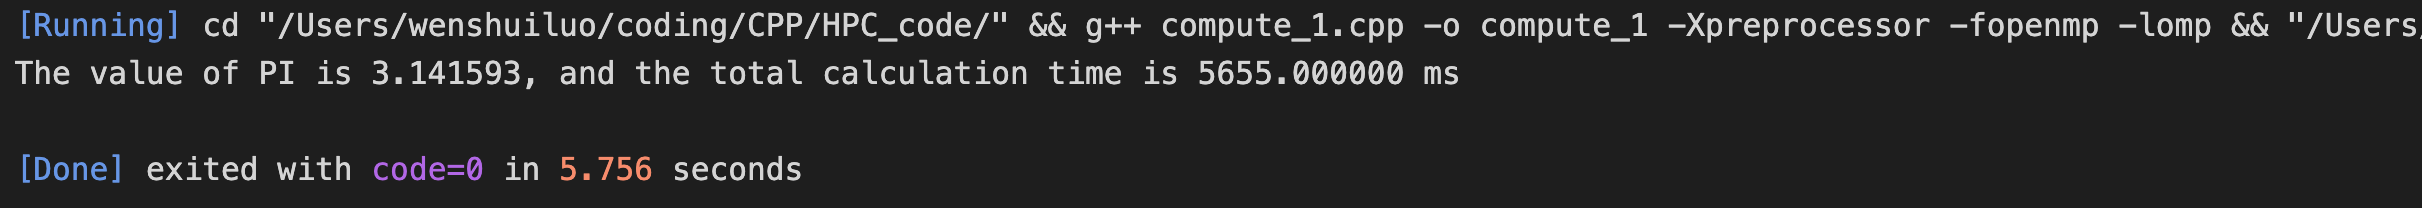
\includegraphics[width=1.0\textwidth]{result4.png}
			\caption{(2)未采用并行方法执行的结果}
		\end{figure}
		
		\begin{figure}[htbp]
			\centering
			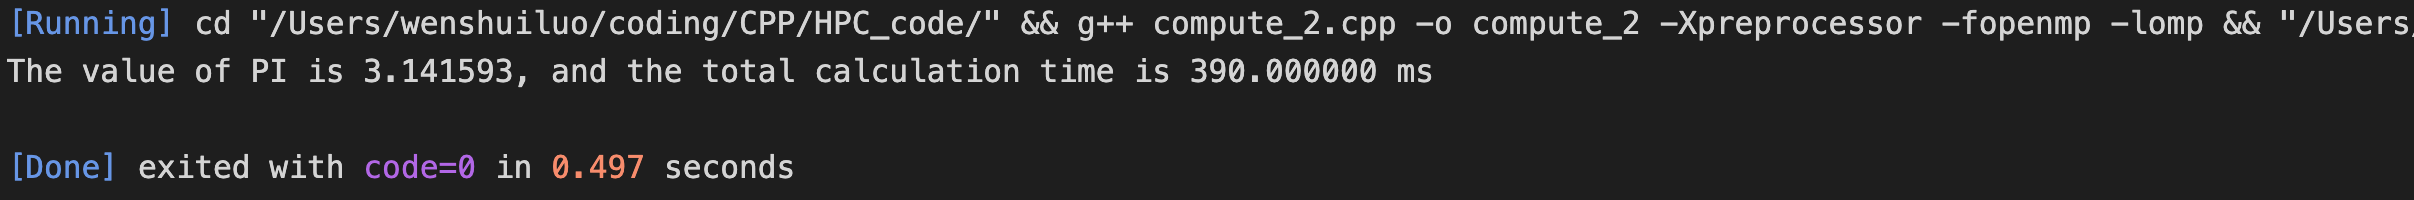
\includegraphics[width=1.0\textwidth]{result5.png}
			\caption{(2)采用并行方法执行的结果}
		\end{figure}

		从中可见未执行并行计算的程序计算时间长达5655ms,并行计算的程序执行时间只有390ms,性能上是未并行程序的十几倍。极大地缩短了计算时间。

	
\end{document}
